\section{Motivation}

\begin{frame}{Motivation}

\begin{itemize}
 \item Given a type $\tau$, how many \textbf{closed} terms can recive $\tau$ in TA$_{\lambda}$?\\[0.5cm]
 \item How many are in a $\beta$-normal form?\\[0.5cm]
 \item The algorithm of Ben-Yelles (1979) answers the 'how many' question for closed $\beta$-normal forms\\[0.5cm]
 \item By the Curry-Howard correspondence, we will have a decision procedure for the Intuitionist Implicational Logic 
\end{itemize}


 
\end{frame}

\section{Inhabitants}

\begin{frame}{Inhabitants classes}

\begin{mydef}[Inhabitants]
\begin{itemize}
 \item \textbf{untyped inhabitant}: closed $M$ such that $\vdash_{\lambda} M : \tau$
 \item \textbf{typed inhabitant}: closed $M^{\tau}$
\end{itemize}
\end{mydef}

\begin{itemize} 
 \item[(i)]  \textbf{\textit{Habs}$_u(\tau)$}: untyped inhabitants
 \item[(ii)] \textbf{\textit{Habs}$_t(\tau)$}: typed inhabitants
 \item[(iii)]\textbf{\textit{Nhabs}$_u(\tau)$}: untyped inhabitants in a $\beta$-normal form
 \item[(iv)]\textbf{\textit{Nhabs}$_t(\tau)$}: typed inhabitants in a $\beta$-normal form
 \item[(v)]\textbf{\textit{Nhabs}$_{\eta}(\tau)$}: typed $\beta\eta$-normal inhabitants
 \item[(vi)]\textbf{\textit{Princ}$(\tau)$}: principal inhabitants
 \item[(vii)]\textbf{\textit{Nprinc}$(\tau)$}: principal inhabitants in a $\beta$-normal form
 \item[(viii)]\textbf{\textit{Nprinc}$_{\eta}(\tau)$}: principal inhabitants in a $\beta\eta$-normal form
\end{itemize}

\end{frame}

\begin{frame}{Typed $\beta$-nf's}

\begin{lem}[Structure of a typed $\beta$-nf]\label{8A5}
 Let $\Gamma$ be a type context. Every $\beta$-nf $N^{\alpha} \in \mathbb{TT}(\Gamma)$ can be expressed uniquely in the form:\\[0.3 cm]
 
\begin{itemize}
 \item[(i)] ($\lambda x_1^{\tau_1} ... \,x_m^{\tau_m} \, . \,
   (v^{(\rho_1 \rightarrow \cdots \rho_n \rightarrow \tau^*)} M^{\rho_1}_1 \cdots
   M^{\rho_n}_n)^{\tau^*})^{(\tau_1 \rightarrow \cdots \tau_m \rightarrow \tau^*)}$ \\where $m \geq 0$, $n \geq 0$, and\\[0.3 cm]
   

 \item[(ii)] $ \tau \equiv \tau_1 \rightarrow \cdots \tau_m \rightarrow \tau^*$ \\ for some $\tau^*$, possibly composite, and \\[0.3 cm]
 

 \item[(iii)] each $M^{\rho_j}_j$ is a $\beta$-nf that is typed relative to  $\Gamma \cup \{x_1 : \tau_1,\cdots, x_m : \tau_m\}$
\end{itemize}
\end{lem}

\end{frame}


\begin{frame}{Typed $\beta$-nf's}
\begin{proof}[Induction in $N^{\cancel{\alpha}}$:]
\begin{itemize}
 \item[(IB)] : $N^{\alpha} \equiv x^{\alpha}$, $x$ is in $\beta$-nf and $x \in \mathbb{TT}(\Gamma)$
 \item[(Case 1)] : $N^{\cancel{\alpha}} \equiv A B$
 
 $A$ is not an abstraction because if it was, $A B$ would not be in $\beta$-nf. 
 $A \equiv v H_1 \cdots H_k$. And by IH $A^{\gamma \rightarrow \alpha} \in \mathbb{TT}(\Gamma_1)$ and $B^{\gamma} \in \mathbb{TT}(\Gamma_2)$. 
 
 So using $\alpha$ equivalence to avoid clashes,
 
 $N^{\alpha} \in \mathbb{TT}(\Gamma_1 \cup \Gamma_2)$ is in the form
 $(v^{\rho_1\rightarrow \cdots \rho_k \rightarrow \gamma \rightarrow \alpha} H^{\rho_1}_1 \cdots
 H^{\rho_k}_k B^{\gamma})^{\alpha}$
 
 \item[(Case 2)] : $N^{\cancel{\alpha}} \equiv \lambda x \, . \, A$
 
 By IH, $A^{\gamma} \in \mathbb{TT}(\Gamma_1)$ and
it has the anounced form. 

Thus, $(\lambda x^{\omega}\, . \,
A^{\gamma})^{\omega \rightarrow \gamma} \in \mathbb{TT}(\Gamma_1 - \{x:
\omega\})$ has the same form.
\end{itemize} 
\end{proof}
\end{frame}



\begin{frame}{Long $\beta$-nf's}

 \begin{mydef}[Long $\beta$-nf's]
The $\beta$-nf $M^{\tau}$ is \textbf{long} or \textbf{maximal} 
iff each component with form ($z\, P_1 \cdots P_n)(n \geq 0)$ that is
not in a function position has atomic type.
\end{mydef}
\vspace*{0.3cm}

\begin{notation}[$Long(\tau)$]
 long normal inhabitants of $\tau$ (typed or untyped)
\end{notation}
\vspace*{0.3cm}

\begin{exa}[$\tau \equiv ((a \to b) \to c) \to (a \to b) \to c$]
\begin{itemize}
 \item[(i)] $M^{\tau} \equiv \lambda x^{(a\to b) \to c} \, y^{a \to b} \cdot x^{(a \to b) \to c} \, y^{a \to b}$ 
 \item[(ii)] $N^{\tau} \equiv \lambda x^{(a\to b) \to c} \, y^{a \to b} \cdot x^{(a \to b) \to c} \, (\lambda z \cdot y^{a \to b}\, z^a)$ \checkmark
\end{itemize}
\end{exa}

\end{frame}

\begin{frame}{Long $\beta$-nf's} 
 \begin{lem}[Completeness of $Long(\tau)$] \label{8A8} Every normal inhabitant of $\tau$ can be $\eta$-expanded to a long normal inhabitant of $\tau$.
And this long inhabitant is unique (modulo $\equiv_{\alpha}$); ie
\begin{center}
$\{M^{\tau}, N^{\tau} \in \mbox{Long}(\tau) \mbox{ and } M^{\tau} =_{\eta} N^{\tau}\} \Longrightarrow  M^{\tau} \equiv_{\alpha} N^{\tau}$ 
\end{center}
In particular
\begin{center}
 Nhabs$(\tau) = \emptyset \Longleftrightarrow$ Long$(\tau) = \emptyset$. 
\end{center}


\end{lem}

\begin{figure}[h]
   \centering
   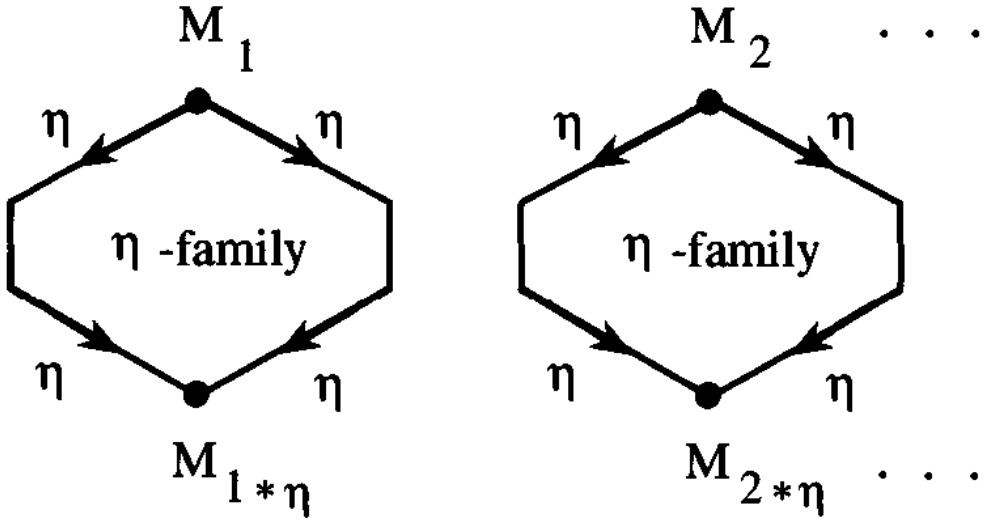
\includegraphics[scale=0.3]{fig1.png}
\end{figure}
\end{frame}

\begin{frame}{Long $\beta$-nf's}


\begin{proof}
 \begin{itemize}
  \item Let $P^{\tau} \in Nhabs(\tau)$
  \item $\eta$-expand $P^{\tau}$ to $P^{\tau +} \in Long(\tau)$. We must show that $P^{\tau +}$ is unique
  \begin{center}
   $M^{\tau} \in Long(\tau), \,\,\, M^{\tau}\twoheadrightarrow_{\eta} P^{\tau} \,\,\,\,\Longrightarrow \,\,\,\,M^{\tau} \equiv_{\alpha} P^{\tau +}$
  \end{center}
  \item suppose $P^{\tau}$ contains a component $(y\,Q_1\cdots Q_n)^{\sigma}$ that is not long
  \item it is not in function position and $\sigma \equiv \sigma_1 \to \cdots \to \sigma_k \to a\,\,\,\,\, (k \geq 1)$ 
  \item given new variables $z_1, ..., z_k$ not occuring in $P^{\cancel{\tau}}$, replace this component by
  \begin{center}
   $(\lambda z_1^{\sigma_1}\,...\, z_k^{\sigma_k} \cdot ((y\,Q_1\cdots Q_n)^{\sigma}\, z_1^{\sigma_1}\cdots z_k^{\sigma_k})^a)^{\sigma}$
  \end{center}
  \item[(i)] Make similar replacements until there are no short components in $P^{\tau}$. Call the result $P^{\tau +}$
  \item[(ii)] this replacements are $\eta$-expansions and its result is still a $\beta$-nf
  \item[(iii)] the proof is complete with rotine induction in $|P^{\tau}|$
 \end{itemize}
\end{proof}

\end{frame}

\begin{frame}{Long $\beta$-nf's}
 \begin{itemize}
  \item[(i)] Each replacement may introduce new short components with types $\sigma_1, ..., \sigma_k$, but these types are shorter than $\sigma$ so
   the replacement process will terminate\\[0.3cm]
  \item[(ii)] in $(\lambda z_1^{\sigma_1}\,...\, z_k^{\sigma_k} \cdot ((y\,Q_1\cdots Q_n)^{\sigma}\, z_1^{\sigma_1}\cdots z_k^{\sigma_k})^a)^{\sigma}$ the 
              $\beta$-reductions could ocurr just inside $Q_1\cdots Q_n$, but it is contraditory with the fact that $(y\,Q_1\cdots Q_n)^{\sigma}$ is $\beta$-nf\\[0.3cm]
  \item[(iii)] Now the induction over $|P^{\tau} \equiv \lambda x_1^{\tau_1} ... \,x_m^{\tau_m} \, . \, v\, M^{\rho_1}_1 \cdots M^{\rho_n}_n|$:\\[0.2 cm]
     \begin{itemize}
      \item By IH, for each $j$, $Long(\tau)\,\,\, \mbox{\reflectbox{$\in$}} \,\,\,M_j^{\rho_j +} \!\! \twoheadrightarrow_{\eta} \!M_j^{\rho_j}$ and $M_j^{\rho_j +}$ is unique\\[0.3 cm]
      \item $P^{\tau +} \equiv \lambda x_1^{\tau_1} ... \,x_m^{\tau_m} \, z_1^{\sigma_1}\,...\, z_k^{\sigma_k} . \, v\, M^{\rho_1 +}_1 \cdots M^{\rho_n +}_n \, z_1^{\sigma_1}\,...\, z_k^{\sigma_k}$\\[0.3 cm]
      \item $P^{\tau +} \in Long(\tau), \,\,\, P^{\tau +}\twoheadrightarrow_{\eta} P^{\tau}$\\[0.3 cm]
      \item $M^{\tau} \in Long(\tau), \,\,\, M^{\tau}\twoheadrightarrow_{\eta} P^{\tau} \,\,\,\,\Longrightarrow \,\,\,\,M^{\tau} \equiv_{\alpha} P^{\tau +}$\\
     \end{itemize}
 \end{itemize}

\end{frame}



\begin{frame}
 
 \begin{mydef}[Cardinality of $\mathbb{S}$]
 The number of members (modulo $\equiv_{\alpha}$) of a set $\mathbb{S}$.
 \begin{itemize}
  \item $\#(Nhabs(\tau))  \longleftrightarrow  \#(\tau)$
  \item $\#(Nhabs_{\eta}(\tau)) \longleftrightarrow \#_{\eta}(\tau)$
 \end{itemize}
\end{mydef}
 
 \begin{notation}
  $\{M^{\tau}\}_\eta \equiv$ the set of all terms that $\eta$-reduces from $M^{\tau}$ 
  \end{notation}

\begin{lem}\label{8A10}

    \begin{itemize}


           \item[(i)] The $\eta$-families  $\{M^{\tau}\}_\eta$ of long typed terms $M^{\tau}$ 
             patitions $Nhabs(\tau)$ into non-overlapping finite subsets. Each $\eta$-family contain one long
             member and one $\beta \eta$-nf.

        \item[(ii)] $\#_{\eta}(\tau) = \#(Long(\tau))$
        
        \item[(iii)] $\#(\tau)$ is infinte, finite or zero according to 
         
         $\#_\eta(\tau)$ is infinite, finite or zero.

      \end{itemize}
\end{lem}

\end{frame}

\begin{frame}

\begin{proof}
 \begin{itemize}
  \item $M^{\tau} \in \mathbb{TT}(\Gamma), \,\,\,\{M^{\tau}\}_{\eta}$ is finite (by the lemma \textbf{CR}$_{\eta}$) 
  \item $\{M^{\tau}\}_{\eta} \subseteq \mathbb{TT}(\Gamma)$ (lemma \textbf{5B7.1})
  \item if $M^{\tau}$ is a $\beta$-nf then so are all members of $\{M^{\tau}\}$ (typed analogue of the lemma \textbf{1C9.3})
 \begin{center}
  $M^{\tau} \in Nhabs(\tau) \,\,\,\Longrightarrow \,\,\,\{M^{\tau}\}_{\eta} \subseteq Nhabs(\tau)$
 \end{center}
  \item if $M^{\tau}$ is a $\beta$-nf its $\eta$-family contains exactly one $\beta\eta$-nf (typed analogue of the lemma \textbf{1C9.3})
  \item each normal inhabitant of $\tau$ is in the $\eta$-family of exactly one long normal inhabitant (by the lemma \ref{8A8})
  \item And by the \textbf{WN} lemma, $\#(\tau)$ is infinte, finite or zero according to  $\#_\eta(\tau)$ is infinite, finite or zero.
 \end{itemize}
 \end{proof}
 
 
\end{frame}


\begin{frame}
 \begin{lem}
    Let $M^{\tau+}$ be the unique member of $Long(\tau)$ to which
    $M^{\tau}$ $\eta$-expands. 

  \begin{center}
       $M^{\tau} \in Nprinc(\tau) \Longrightarrow M^{\tau+} \in Nprinc(\tau)$
   \end{center}
\end{lem}

\begin{proof}
\begin{itemize}
  \item $\eta$-expansion in the lemma \ref{8A8} preserves principality
  \item there the types of $z_1, ..., z_k$ are determined by the type $\tau$ of the component that is replaced 
\end{itemize}
 
\end{proof}

\end{frame}

\begin{frame}

\begin{figure}[h]
   \centering
   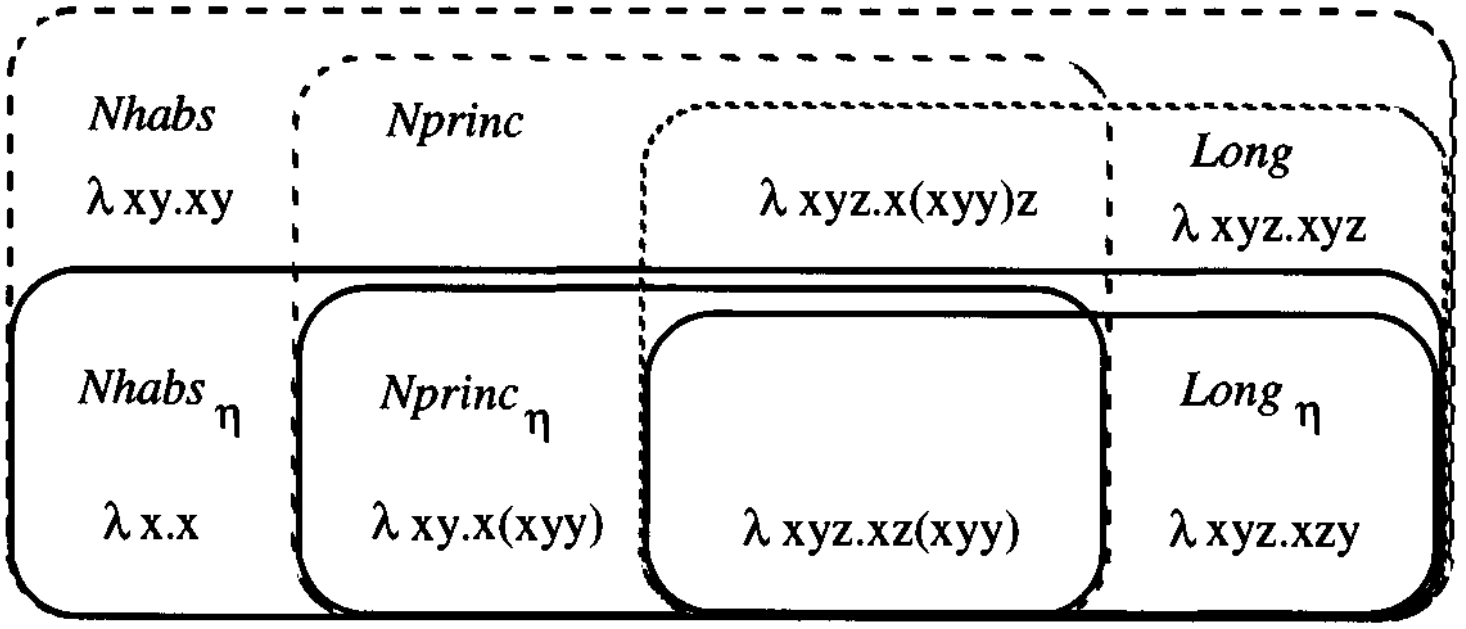
\includegraphics[scale=0.3]{fig2.png}
\end{figure}

\begin{center}
$\tau \equiv (a\to a\to a)\to a \to a \to a$\\[0.5cm]

$
\begin{array}{rlcl}
\mbox{(i)} & \lambda x^{a\to a \to a} \cdot x^{a\to a \to a} & \in & Nhabs_{\eta} - (Nprinc \cup Long)\\ 
\mbox{(ii)} & \lambda x^{a\to a \to a} \, y^{a} \cdot (x\,y)^{a \to a}& \in & Nhabs - Nhabs_{\eta} - (Nprinc \cup Long)\\ 
\mbox{(iii)} & \lambda x^{a\to a \to a} \, y^{a} \, z^{a} \cdot (x\,y\,z)^{a}& \in & Long - Nhabs_{\eta} - Nprinc\\
\mbox{(iv)} & \lambda x^{a\to a \to a} \, y^{a} \cdot (x\,(x\,y\,y))^{a \to a}& \in & Nhabs_{\eta} - Long_{\eta} \\ 
\mbox{(v)} & \lambda x^{a\to a \to a} \, y^{a} \, z^{a} \cdot (x\,(x\,y\,y)\,z)^{a}& \in & Nprinc \cap Long - Nhabs_{\eta} \\ 
\mbox{(vi)} & \lambda x^{a\to a \to a} \, y^{a} \, z^{a} \cdot (x\,z\,(x\,y\,y))^{a}& \in & Nprinc_{\eta} \cap  Long_{\eta}\\ 
\mbox{(vii)} & \lambda x^{a\to a \to a} \, y^{a} \, z^{a} \cdot (x\,z\,y)^{a}& \in &  Long_{\eta} - Nprinc_{\eta}\\ 
\end{array}
$
\end{center}

 
\end{frame}

\begin{frame}
\frametitle{Remarks}
 \begin{itemize}
  \item $Habs(\tau) \neq \emptyset \Longleftrightarrow Nhabs(\tau) \neq \emptyset\,\,\,\,\,$ [\textbf{WN}]
  \item $Habs(\tau) \neq \emptyset \Longleftrightarrow Princ(\tau) \neq \emptyset\,\,\,\,\,\,\,$ [\textbf{converse PT}]
  \item $Habs(\tau) \neq \emptyset \,\,\,{\color{red}\nRightarrow} \,\,\,Nprinc(\tau) \neq \emptyset$
  \item $Princ(\tau) \neq \emptyset \,\,\,{\color{red}\nRightarrow} \,\,\, Nprinc(\tau) \neq \emptyset$
 \end{itemize}

\begin{block}{} 
$\tau$ may have an inhabitant $M$, enven a principal one, such that $PT(M)$ changes when $M$ is reduced to $M*_{\beta}$. 
\end{block}

\begin{exa}[$\tau \equiv a \to a \to a$]
\begin{itemize}
 \item $Nhabs(\tau) = \{\lambda xy \cdot x, \lambda xy \cdot y\}$, but neither of these is principal
 \item But there is a non-normal principal inhabitant: $(\lambda xyz \cdot \mbox{\textbf{K}}(xy)(xz))$\textbf{I}
\end{itemize}


\end{exa}
 
 
\end{frame}




\section{Search strategies}

\begin{frame}
 
 \begin{lem}
   Every type $\tau$ has the form:
   \begin{center}
         $\tau \equiv \tau_1 \rightarrow \cdots \rightarrow \tau_m \rightarrow e$
   \end{center}
  with $m \geq 0$ and $e$ atomic.
\end{lem}
 
\begin{proof}
 \begin{itemize}
  \item if $\tau \equiv a$ then $m = 0$ OK
  \item if $\tau \equiv \sigma \to \rho$ por IH\\
   $\sigma \equiv \sigma_1 \to \cdots \to \sigma_n \to e_{\sigma}$\\
   $\rho \equiv \rho_1 \to \cdots \to \rho_k \to e_{\rho}$\\
   \begin{center}
   $\tau \equiv (\sigma_1 \to \cdots \to \sigma_n \to e_{\sigma}) \to \rho_1 \to \cdots \to \rho_k \to e_{\rho}$
   \end{center}
   
 \end{itemize}
 
\end{proof}
 
\end{frame}


\begin{frame}

\begin{notation}[for $\tau \equiv \tau_1 \rightarrow \cdots \rightarrow \tau_m \rightarrow e$]
\begin{itemize}
 \item The occurrences of $\tau_1,...,\tau_n$ and $e$ will be called \textbf{premises} and \textbf{conclusion} (or \textbf{tail}) of $\tau$\\[0.3cm]
 
 \item $m$ will be called the \textbf{arity} of $\tau$\\[0.3cm]
 
 \item Two type-occurrences will be called \textbf{isomorphic} iff they are occurrences of the same type\\[0.3cm]
 
 \item If the tail-components of $\sigma$ and $\tau$ are isomorphic we may say:
\begin{center}
 $Tail(\sigma) \cong Tail(\tau)$ 
\end{center}
 
\end{itemize}

\end{notation}
  
\begin{mydef}[nf-schemes]
 A nf-scheme is a $\beta$-nf that may contain meta-variables under restrictions:
 \begin{itemize}
  \item[(i)] each nf-scheme is a $\beta$-nf without bound-variables clashes
  \item[(ii)] meta-variables do not bind ($\lambda V$ is forbidden)
  \item[(iii)] in a composite nf-scheme meta-variables only occur in argument positions
  \item[(iv)] each meta-variable in a nf-scheme occurs only once
 \end{itemize}
\end{mydef}
  
\end{frame}


\begin{frame}
\frametitle{Comments}
Let $\tau$ be any type; say $\tau$ has form
\begin{center}
 $\tau \equiv \tau_1 \rightarrow \cdots \rightarrow \tau_m \rightarrow e \,\,\,\,\,\,\, (m \geq 0, e \mbox{ an atom})$
\end{center}
and let $M^{\tau}$ be any $\beta$-nf with type $\tau$. By the lemma \ref{8A5}, $M^{\tau}$ has form
\begin{center}
 $\lambda x_1^{\tau_1} ... \,x_k^{\tau_k} \, . \,
   (v^{(\rho_1 \rightarrow \cdots \rho_n \rightarrow \tau^*)} M^{\rho_1}_1 \cdots
   M^{\rho_n}_n)^{\tau^*})^{(\tau_1 \rightarrow \cdots \tau_k \rightarrow \tau^*)}$
\end{center}
where $0 \leq k \leq m$ and $\tau^* \equiv \tau_{k+1} \to \cdots \to \tau_m \to e$.\\[0.3 cm]
If $M^{\tau} \in Long(\tau)$, then
\begin{itemize}
 \item[(i)] $k = m$ and $\tau^* \equiv e$
 \item[(ii)] the types of $x_1,..,x_m$ coincide with the premises of $\tau$
 \item[(iii)] the tail of the type of $v$ is isomorphic to $Tail(\tau)$
 \item[(iv)] if $M^{\tau}$ is closed then $m \geq 1$ and $v$ is an $x_i \,\,\, (1 \leq i \leq m)$ and
 \begin{center}
  $\tau_i \equiv \rho_1 \to \cdots \to \rho_n \to e$
 \end{center}

\end{itemize}

\end{frame}

\section{Examples of search} 

\begin{frame}
\frametitle{Example $\#(\tau) = 1$}
\begin{block}{ $\tau \equiv (a \to b \to c) \to (a \to b) \to a \to c$}
has exactly one normal inhabitant
\end{block}
\begin{block}{\textbf{S}$^{\tau} \equiv \lambda x^{a \to b \to c}\,y^{a \to b}\,z^a\cdot x\,z\,(y\,z)$}
is its normal inhabitant and is $\in Long(\tau) \cap Princ(\tau)$
\end{block}

\vspace*{0.3 cm}

 \begin{itemize}
  \item[Step 1.] Start by proving that $Long(\tau) = \{\mbox{\textbf{S}}^{\tau}\}$, and looking at the structure of $\tau$; 
  by following the previous comments; we must have:\\[0.2 cm] 
  
			      $\left\{\begin{array}{lcl}
                               m & = & 3 \\
                               e & \equiv & c \\
                               \tau_1 & \equiv & a \to b \to c \\
                               \tau_2 & \equiv & a \to b \\
                               \tau_3 & \equiv & a
                              \end{array}\right.$

 \end{itemize}

 \end{frame}
 
\begin{frame}
\frametitle{Example $\#(\tau) = 1$}
\begin{block}{$M^{\tau} \equiv (\lambda x_1^{\tau_1}\,x_2^{\tau_2}\,x_3^{\tau_3}\cdot(v^{(\rho_1 \to \cdots \rho_n \to c)}\,M_1^{\rho_1}\cdots M_n^{\rho_n})^c)^{(\tau_1 \to \tau_2 \to \tau_3 \to c)} $} 
$\in Long(\tau)$ and has three inital abstracted variables 
\end{block}
\begin{itemize}
 \item By the item (iv) of the previous comments, $v$ must be one of $x_1, x_2, x_3$ whose type's tail is isomorphic to $Tail(\tau) \equiv c$
 \item Then the unique possibly choose is $v \equiv x_1$
 \item $x_1$ must be followed by exactly two arguments, and hence $M$ must have form:
\end{itemize}

\begin{equation}
M \equiv \lambda x_1^{a\to b\to c}\,x_2^{a\to b}\,x_3^a \cdot x_1^{a \to b \to c}\,{\color{red}U^a}\,{\color{blue}V^b}
\end{equation}
\end{frame}

\begin{frame}
\frametitle{Example $\#(\tau) = 1$} 
\begin{itemize}
 \item[Step 2.] Search for suitables ${\color{red}U^a}$ and ${\color{blue}V^b}$\\[0.3cm]
 
 \begin{itemize}
  \item[(i)] by the comments (i), ${\color{red}U^a} \equiv (w\,P_1 \cdots P_r)^a \,\,\,\,\,\,\, (r \geq 0)$
  \item[(ii)]$w$ is an $x_i$ whose type's tail is isomorphic to the tail of the type of ${\color{red}U^a}$
  \item[(iii)] this tail is an occurrence of ${\color{red}a}$, so $w \equiv x_3$
  \item[(iv)] since $x_3$ has no premises so $r = 0$ and \\[0.3cm]
 \end{itemize}
\begin{equation}
 {\color{red}U^a} \equiv x_3^a
\end{equation}
  \begin{itemize}
   \item[(i)] $b$ is an atom then ${\color{blue}V^b}$ cannot be an abstracted
   \item[(ii)] its head must be $x_i$ whose type's tail is an ocurrence of ${\color{blue}b}$
   \item[(iii)] the only possibility is $x_2$
   \item[(iv)] $x_2$ allows only one argument, so \\[0.3cm]
\begin{equation}
 {\color{blue}V^b} \equiv x_2^{a \to b} \, {\color{magenta}W^a}
\end{equation}
  \end{itemize}
\end{itemize}
 
\end{frame}

\begin{frame}
 \frametitle{Example $\#(\tau) = 1$}
\begin{itemize}
 \item[Step 3.] Just as for ${\color{red}U^a}$, the only possibility for ${\color{magenta}W^a}$ is\\[0.3cm]
\begin{equation}
  {\color{magenta}W^a} \equiv x_3^a
\end{equation}
\end{itemize}

\textbf{Conclusion.}

\begin{block}{\begin{center}
               \textbf{S}$^{\tau} \equiv \lambda x_1^{a \to b \to c}\,x_2^{a \to b}\,x_3^a\cdot x_1\,x_3\,(x_2\,x_3)$
              \end{center}}
\begin{center}
there is at most one term (modulo $\equiv_{\alpha}$) in $Long(\tau)$
\end{center}
\end{block}
\begin{itemize}
 \item By the lemma \ref{8A10} and the fact that \textbf{S}$^{\tau}$ is a $\beta\eta$-nf:
 $Nhabs(\tau) = \{S^{\tau}\}$
 \item By the PT algorithm $\tau$ is a principal type of \textbf{S}$^{\tau}$: 
 $Nprinc(\tau) = \{S^{\tau}\}$ 
\end{itemize}

\end{frame}


\begin{frame}
\frametitle{Example $\#(\tau) = m$}
\begin{block}{ $\tau \equiv a \to \cdots \to a \to a\,\,\,\,\,\,\, (m+1 \,a\mbox{'s})$}
for each $m \geq 2$, has exactly $m$ normal inhabitants
\end{block}
\begin{block}{$\Pi^m_i \equiv \lambda x_1^a\,...\,x_m^a\cdot x_i^a\,\,\,\,\,\,\,(1 \leq i \leq m)$}
is its normal inhabitants and is $\in Long(\tau) - Princ(\tau)$. They are called \textbf{projectors} or \textbf{selectors}
\end{block}
 
\end{frame}


\begin{frame}
 \frametitle{Example $\#(\tau) = m$}

\begin{proof}
 \begin{itemize}
  \item By the previous comments, any $M^{\tau} \in Long(\tau)$ must have form\\[0.3 cm]
\begin{center}
 $M^\tau \equiv \lambda x_1^a\,...\, x_m^a \cdot v\,V1 \cdots V_n$
\end{center}
  \item $v \equiv x_i$ for some $i\leq m$
  \item But the types of $x_1, ..., x_m$ have no premises, so $n = 0$. Hence\\[0.3 cm]
\begin{center}
 $M^{\tau} \equiv \lambda x_1^a\,...\,x_m^a \cdot x_i^a$
\end{center}
  \item All selectors are in $Long(\tau)$ and they are $\beta\eta$-nfs. Then by the lemma \ref{8A10}\\[0.3 cm]
\begin{center}
 $Nhabs(\tau) = Long(\tau)$
\end{center}
  \item $m \geq 2$, so by the PT algorithm no selector is in $Nprinc(\tau)$\\[0.3 cm]
\begin{center}
 $Nprinc(\tau) = \emptyset$ 
\end{center}


\end{itemize}
\end{proof}

 
\end{frame}


\begin{frame}
\frametitle{Example $\#(\tau) = 0$}
\begin{itemize}
 \item[(Ex1)] No atomic type has inhabitants
\begin{proof}
 \begin{itemize}
  \item Every type with an inhabitant has a normal one
  \item But every type with a closed normal inhabitant has arity $m \geq 1$  (comments (iv))
 \end{itemize}
\end{proof}
 
 \item[(Ex2)] No type that is skeletal has inhabitants
\begin{proof}
  \begin{itemize}
   \item Let $\tau$ be skeletal and $\tau \equiv \tau_1 \to ... \to \tau_m \to e\,\,\,(m \geq 1)$
   \item If $\tau$ had inhabitants it would have at least one long normal one by the lemma \ref{8A8}
   \item This inhabitant would have form
    $\lambda x_1\,...\,x_m\cdot x_i\,M_1\cdots M_n$
   \item $x_i$ having type $\tau_i$ and the tail of $\tau_i$ being an occurrence of $e$
   \item $\tau$ is skeletal so $e$ cannot occur in any $\tau_i$. Hence $\tau$ has no inhabitants
  \end{itemize}
\end{proof}
\end{itemize}

\end{frame}

\begin{frame}{Example $\#(\tau) = 0$}
\begin{itemize}
  \item[(Ex3)] \textbf{The Peirce's law} ($\tau \equiv ((a \to b) \to a) \to a$) has no inhabitants
 \begin{proof}
  \begin{itemize}
   \item If $M^{\tau} \in Long(\tau)$ then, by the comments, 
   \begin{center}
       $M^{\tau} \equiv \lambda x^{(a\to b) \to a} \cdot v\,U_1\cdots U_n\,\,\,\,\,(n \geq 0)$
   \end{center}
   \item $v \equiv x$, since $M^{\tau}$ is closed. Hence $n = 1$
   \begin{center}By the remarks and the lemma \ref{8A8} 
    \begin{center}\
    $Long(\tau) = \emptyset \Rightarrow Nhabs(\tau) = \emptyset \Rightarrow Habs(\tau) = \emptyset$
    \end{center}
       $M^{\tau} \equiv \lambda x^{(a\to b) \to a} \cdot x^{(a\to b) \to a}\,U^{a\to b}$ 
   \end{center}
    \item Since $a\to b$ has just one premise:
   \begin{center}
    $U^{a\to b} \equiv \lambda y^a \cdot (w\,V_1\cdots V_r)^b\,\,\,\,\, (r \geq 0)$
   \end{center}
    \item $M^{\tau}$ is closed so $w$ must be $x$ or $y$
    \item $w$ must have a type whose tail is an ocurrence of $b$, but neither $x$ nor $y$ has such type
    \item 
  \end{itemize}
 \end{proof}
\end{itemize}
\end{frame}

\begin{frame}
\frametitle{More examples of search}



% $\begin{array}{lcll}
%  P_0  & \equiv & \lambda x \cdot x\,\mbox{\textbf{I}} \\ 
%  P_n  & \equiv & \lambda x \cdot x\,(\lambda y_1 \cdot x\,(\cdots (\lambda y_n \cdot x\,\mbox{\textbf{I}}) \cdots )) &  (n \geq 1), \\
%  Q_{n,i} & \equiv & \lambda x \cdot x\,(\lambda y_1 \cdot x\,(\cdots (\lambda y_n \cdot x\,(\lambda z\cdot y_i)) \cdots )) & (n \geq 1, 1 \leq i \leq n)
%  \end{array}
% $
% \vspace*{0.5cm}
% 
% 



$
 \begin{array}{lllll}\hline\hline
 \mbox{\textbf{Type} } \tau             & Nhabs(\tau)         & Long(\tau)        & Nprinc(\tau)       \\\hline
  a\to a                                 & \mbox{\textbf{I}}   & \mbox{\textbf{I}} & \mbox{\textbf{I}} \\
  a\to b\to a                            & \mbox{\textbf{K}}   & \mbox{\textbf{K}} & \mbox{\textbf{K}} \\
 (a\to b)\to (c \to a) \to c \to b       & \mbox{\textbf{B}}   & \mbox{\textbf{B}} & \mbox{\textbf{B}} \\
 (a\to b\to c)\to b\to a\to c            & \mbox{\textbf{C}}   & \mbox{\textbf{C}} & \mbox{\textbf{C}} \\
 (a\to b\to c)\to (a\to b)\to a\to c     & \mbox{\textbf{S}}   & \mbox{\textbf{S}} & \mbox{\textbf{S}} \\
 (a\to a\to b)\to a\to b                 & \mbox{\textbf{W}}   & \mbox{\textbf{W}} & \mbox{\textbf{W}} \\
 (a\to a) \to a \to a                    & \mbox{\textbf{I}}, \bar{0}, \bar{1}, \bar{2}, ... & \bar{0}, \bar{1}, \bar{2}, ... &\bar{2}, ... \\

  \\\hline\hline
 \end{array}
$

\begin{center}
$
\begin{array}{lcllcl}
 \mbox{\textbf{B}} & \equiv & \lambda x y z \cdot x (y z) & \mbox{\textbf{C}} & \equiv &  \lambda x y z \cdot x z y \\
 \mbox{\textbf{K}} & \equiv & \lambda x y \cdot x &  \mbox{\textbf{I}} & \equiv & \lambda x \cdot x \\
 \mbox{\textbf{S}} & \equiv & \lambda x y z \cdot x z (y z) &  \mbox{\textbf{W}} & \equiv & \lambda x y \cdot x y y \\
 \bar{n} & \equiv & \lambda x y\cdot x^n y
\end{array}
$
\end{center}

\end{frame}

\section{Introduction to the search algorithm}

\begin{frame}{Depth of a term}
\begin{mydef}
 The depth of typed or untyped terms is given by $(m \geq 0)$:
 
 \begin{itemize}
     \item[(i)] $Depth(\lambda x_1\, \cdots \, x_m\, . \, y) = 0$
      \item[(ii)] $Depth(\lambda x_1\, \cdots \, x_m\, . \, y \,M_1 \cdots M_n) = 1+ \underset{1 \leq j \leq n}{Max}\,Depth(M_j)\,\,\,\,\,\,\,$ if $n > 0$
  \end{itemize}
\end{mydef}

\begin{exa}
 \begin{itemize}
  \item $Depth(\lambda u v \cdot u x v x) = Depth(z(\lambda w \cdot y)) = 1$
  \item $Depth(\lambda x \cdot x(z(\lambda w \cdot y))(\lambda u v \cdot u x v x)) = 2$
 \end{itemize}
\end{exa}

\end{frame}

\begin{frame}{Introduction to the search algorithm}
 
 \begin{itemize}
  \item First look for members of $Long(\tau)$ with\\ 
   depth $d = 0$, then $d = 1$, ...\\[0.3 cm]
  \item The output is the sequence  of finite sets $\mathcal{A}(\tau,0),\,\mathcal{A}(\tau,1),\,\mathcal{A}(\tau,2),\,...$ as aproximations of $Long(\tau)$\\[0.3 cm]
  \item Those in $\mathcal{A}(\tau,d)$ will look like typed $\beta$-nf's with depth $\leq d$ but with some 'holes' (meta-variables)\\[0.3 cm]
  \item To construct $\mathcal{A}(\tau,d+1)$ the aproximations in $\mathcal{A}(\tau,d)$ will be extended by replacing their meta-variables with nf-schemes with depth 1
 \end{itemize}

 
\end{frame}

\begin{frame}{The search algorithm}
          It is an algorithm to find Long terms to an type, but with a
          limitaded depth.
          $\mathcal{A}(\tau,0)$

          \begin{itemize}
                 \item[(i)] If $\tau$ is atomic, outputs empty set

                 \item[(ii)] Otherwise, outputs $\{V^{\tau}\}$, where
                   $V$ is a meta-variable
          \end{itemize}
     
\end{frame}

\begin{frame}
          Assume the output of $\mathcal{A}(\tau,d)$ is ready to
          compute $\mathcal{A}(\tau,d+1)$.

          \begin{itemize}
                 \item[(i)] If the output is the empty set or it not
                   contains any meta-variable in any term,
                   stop. $\mathcal{A}(\tau,d+1)$ is undefined and the
                   algorithm just outputs the sequence
                   $(\mathcal{A}(\tau,0), \cdots, \mathcal{A}(\tau,d))$
          \end{itemize}
\end{frame}

\begin{frame}
      \begin{mydef}
            A proper nf-schemes is one that contain some meta-variable
      \end{mydef}

      For each meta-variable $V^{\rho}$ in each proper nf-scheme $X^{\tau}$ in
      $\mathcal{A}(\tau,d))$
      Consider $\rho$ as

      \begin{center}
            $\rho \equiv \sigma_1 \to \cdots \to \sigma_m \to a$
      \end{center}

      List each $\sigma_i$ such that $tail(\sigma_i) \cong a$. For all
      that, define:
      \begin{center}
            $\sigma_i \equiv \sigma_{i,1} \to \cdots \to \sigma_{i,n_i}
            \to a$
      \end{center}

      and
      
      \begin{center}
             $Y^{\rho}_i \equiv \lambda x^{\sigma_1}_1 \cdots
             x^{\sigma_m}_m \cdot (x^{\sigma_i}_i
             V^{\sigma_{i,1}}_{i,1} \cdots V^{\sigma_{i,n_i}}_{i,n_i})^a$
      \end{center}

      where x`s and V`s are new variables and
      meta-variables. $Y^{\rho}$ is called a suitable replacement of $V^{\rho}$.
\end{frame}

\begin{frame}
     List the abstractors tha cover $V^{\rho}$ in orther that they
     occur in $X^{\tau}$ :

     \begin{center}
          $\lambda z^{\zeta_1}_1, \cdots, \lambda z^{\zeta_t}_t$
     \end{center}

     For each $\zeta_j$ such that $tail(\zeta_j) \cong a$ has the
     form:

     \begin{center}
           $\zeta_j \equiv \zeta_{j,1} \to \cdots \to \zeta_{j,h_j}
           \to a$
     \end{center}

     Define:
     \begin{center}
            $Z^{\rho}_j \equiv \lambda x^{\sigma_1}_1 \cdots x^{\sigma_m}_m
     \cdot (z^{\zeta_j}_j V^{\zeta_{j,1}}_{j,1} \cdots
     V^{\zeta_{j,h_j}}_{j,h_j})^a $
     \end{center}

     where x`s and V`s are new variables and
     meta-variables. $Z^{\rho}_j$ is a suitable substitution of $V^{\rho}$
\end{frame}

\begin{frame}
     Each $X^{\tau}$ in $\mathcal{A}(\tau,d)$ generates some lists of suitable
     substitution for all meta-variable in $X^{\tau}$. But if
     $X^{\tau}$ does not have this kind of list, discart it.

     $\mathcal{A}(\tau,d+1)$ is each substitution of meta-variables
     $X^{\tau}$ by there suitable substitution in a list of suitable replacement.
\end{frame}

\begin{frame}{Example}
  \begin{exa}
      $\tau = a \to b \to c$

      $\mathcal{A}(\tau,0) = \{V^{\tau}\}$

      $\mathcal{A}(\tau,1) = \emptyset$
  \end{exa}
\end{frame}

\begin{frame}{Search algorithms properties}
	\begin{lem}
     \begin{enumerate}
           \item Each member of $\mathcal{A}(\tau,d)$ is a closed long
             term typed $\tau$ and is either:
             \begin{itemize}
                     \item a proper nf-scheme with depth d or
                     \item a term with depth d-1
              \end{itemize}
              \item $\mathcal{A}(\tau,d)$ is finite
               \item $Long(\tau,d) \subseteq \mathcal{A}(\tau,0) \cup \cdots
                 \cup\mathcal{A}(\tau,d+1)$
                 \item $Long(\tau) = \bigcup_{d \geq 0} \mathcal{A}_{terms}(\tau,d)$
      \end{enumerate}
      \end{lem}

      \begin{proof}
             \begin{itemize}
                      \item Item 1 and 2 is made by induction in $d$
                      \item Item 3 is kind of that but with new
                        definitions.
                       \item 4 is a corolary
             \end{itemize}
      \end{proof}
      
\end{frame}

\begin{frame}
  \begin{mydef}
        $\mathbb{D}(\tau) = |\tau| \times ||\tau||$

        Where $|\tau|$ is the number of atom occurences and $||\tau||$
        is the number of distinct atom in $\tau$.
  \end{mydef}

  \begin{lem}[Stretching lemma]
      If $Long(\tau)$ has a member $M^{\tau}$ with depth bigger
      than $||\tau||$, so given any integer, there is another one
      bigger than this integer.
   \end{lem}

   \begin{lem}[Shirinking lemma]
            If $Long(\tau)$ has a member $M^{\tau}$ with depth bigger
            than $\mathbb{D}(\tau)$ there is a member $N^{\tau}$

            Such that

            $\mathbb{\tau}-||\tau|| \leq Depth(N^{\tau}) \leq \mathbb{D}(\tau)$
    \end{lem}

\end{frame}


% \section{First conclusions}
% 
% \begin{frame}{First conclusions}
% \begin{itemize}
%  \item The point is searching for \textbf{long normal forms}\\[0.5cm]
%  
%  \item The the \textbf{Search} and the \textbf{Count Algorithms} will work with the idea of \textbf{nf-schemes} and analisis in the term's \textbf{depth}\\[0.5cm]
%  
%  \item Intuitionist implicational logic is consistent in the sense that not all formulae are provable
% \end{itemize}
% \end{frame}
% 



% \section{The search algorithm}
% 
% \begin{frame}
% 
% 
% 
%  
% \end{frame}
% 
% \section{The Counting algorithm}
% 
% \begin{frame}
% 
% 
% 
%  
% \end{frame}
% 